\chapter{Calculated energies for \ce{Li4Mn2O5}}

\begin{figure}[h]
\centering
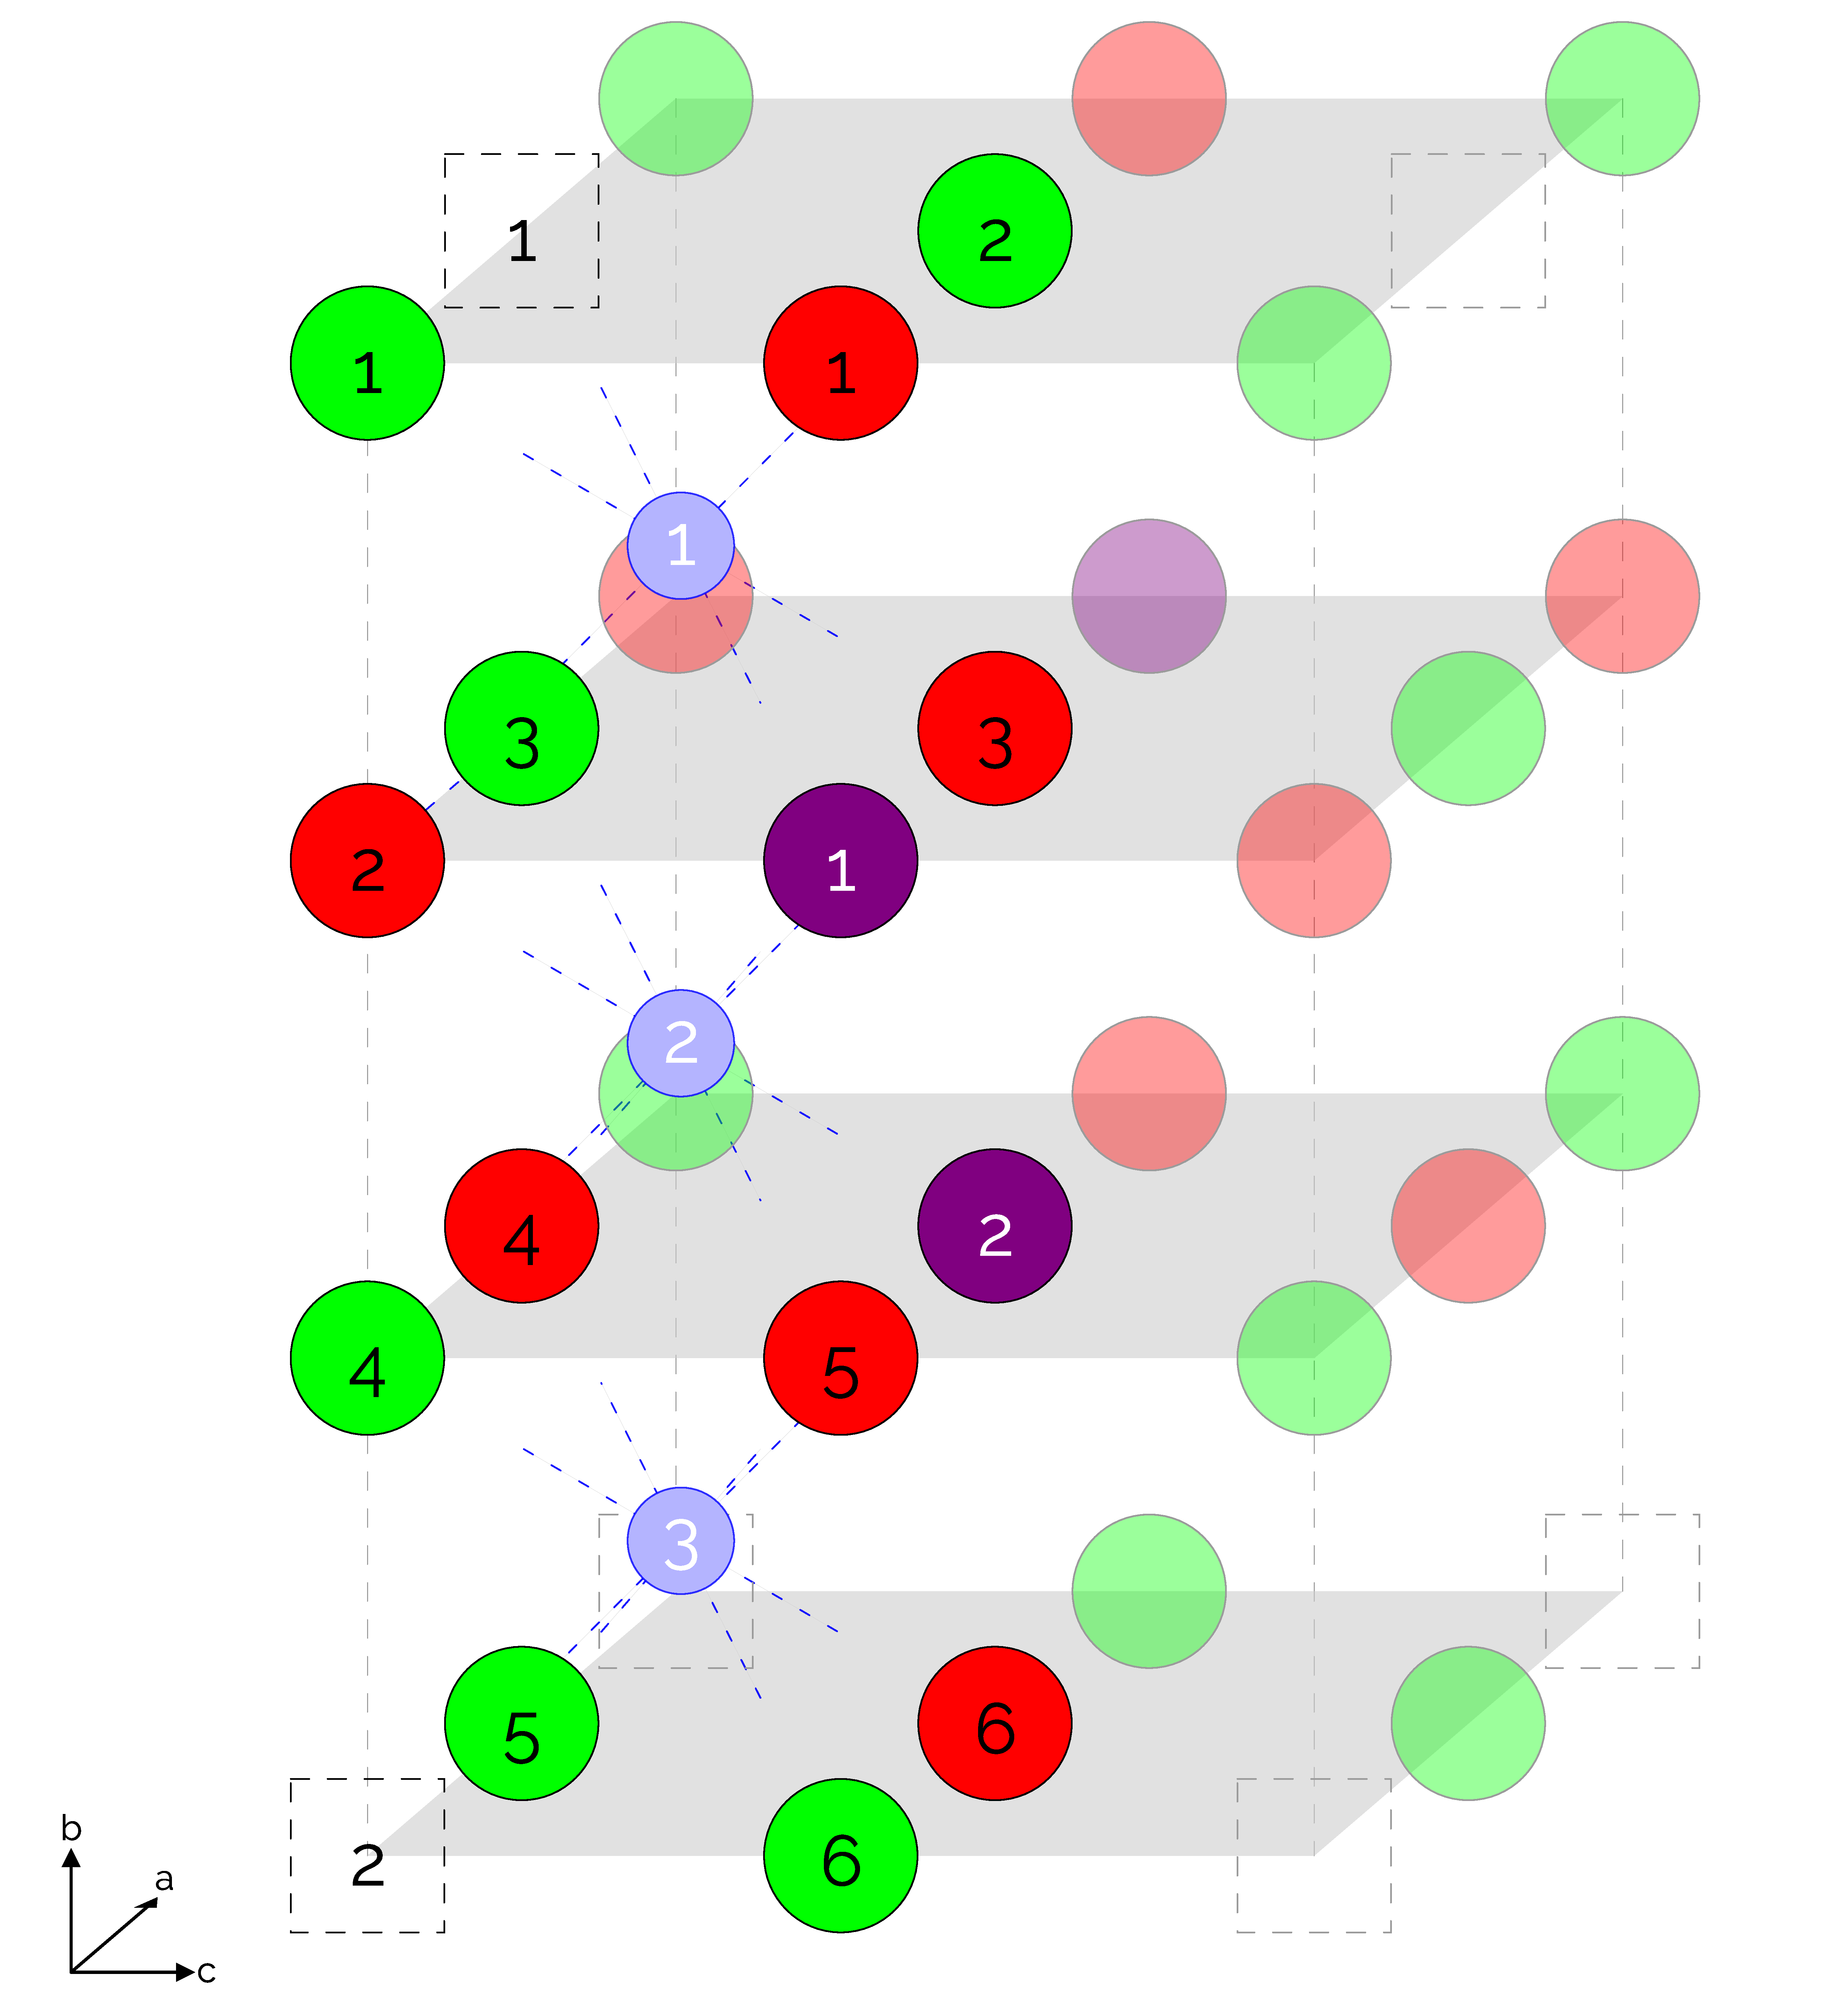
\includegraphics[height = 0.5\textheight]{figures/orderedlabels/orderedlabels}
\caption[Repetition of Figure \ref{fig:orderedlabel} for convenience]{Site labelling scheme for ordered \ce{Li4Mn2O5}. A reflection at either the top or bottom plane yields the structure proposed by \citet{Diaz-Lopez2017}. Li ions: green; Mn ions: purple; O atoms: red.
}
\end{figure}

\newpage
\section{Isolated vacancies}
\paragraph{Kr\"oger-Vink notation for \ce{Li4Mn2O5} vacancies}

\begin{align}
\varnothing &\rightarrow \ce{V^\prime_{Li_n}}\\
\varnothing &\rightarrow \ce{V^{\prime \prime \prime}_{Mn_n}}\\
\varnothing &\rightarrow \ce{V^{\bullet\bullet}_{O_n}}
\end{align}

\vfill
\begin{table}[h]
\centering
\caption{Isolated defect energies for the formation of vacancies in \ce{Li4Mn2O5}}
\begin{tabular}{l *{3}{d{2.3}}}
\toprule
&\multicolumn{3}{c}{Species}\\
\cmidrule(lr){2-4}
\textbf{Site (n)} & \mc{\ce{Li}} & \mc{\ce{Mn}} & \mc{\ce{O}}\\
\midrule
1 & 6.931 & 46.193 & 24.771 \\
2 & 5.573 & 46.193 & 23.240 \\
3 & 7.255 & \tableline & 24.612 \\
4 & 7.255 & \tableline & 23.240 \\
5 & 6.931 & \tableline & 24.612 \\
6 & 5.573 & \tableline & 24.771 \\
\midrule
Minimum & 5.573 & 46.193 & 23.240  \\
\bottomrule
\end{tabular}
\label{tab:vacancies}
\end{table}


\newpage
\section{Isolated interstitial defects}
\paragraph{Kr\"oger-Vink notation for \ce{Li4Mn2O5} interstitial defects}
\begin{align}
\varnothing &\rightarrow \ce{Li^{\bullet}_{i_n}}\\
\varnothing &\rightarrow \ce{Mn^{\bullet\bullet\bullet}_{i_n}}\\
\varnothing &\rightarrow \ce{O^{\prime \prime}_{i_n}}
\end{align}
\vfill
\begin{table}[h]
\centering
\caption{Isolated defect energies for interstitial defects in \ce{Li4Mn2O5}. Numbered sites 1, 2 and 3 refer to the octohedral sites found between layers 1 and 2, 2 and 3, and 3 and 4 respectively. Sites V1 and V2 refer to vacant O sites.}
\begin{tabular}{l *{3}{d{3.3}}}
\toprule
&\multicolumn{3}{c}{Species}\\
\cmidrule(lr){2-4}
\textbf{Site (n)} & \mc{\ce{Li}} & \mc{\ce{Mn}} & \mc{\ce{O}}\\
\midrule
1 & -3.850 & -36.410 & -20.159 \\
2 & -3.799 & -36.712 & -17.087 \\
3 & -3.850 & -36.410 & -20.159 \\
V1 & -2.942 & -36.122 & -20.161 \\
V2 & -2.942 & -36.122 & -20.161 \\
\midrule
Minimum & -3.850 & -36.712 & -20.161  \\
\bottomrule
\end{tabular}
\label{tab:interstitial}
\end{table}

\newpage
\section{Isolated impurities}
\paragraph{{\color{red}Kr\"oger-Vink notation for impurities in \ce{Li4Mn2O5}}}

\begin{align}
\varnothing &\rightarrow \ce{V^{\prime \prime \prime}_{Mn_n}} + \ce{Li^\prime_{Mn_n}} \\
\varnothing &\rightarrow \ce{V^{\prime \prime \prime}_{Mn_n}}\\
\varnothing &\rightarrow \ce{V^{\bullet\bullet}_{O_n}}
\end{align}

\vfill
\begin{table}[h]
\centering
\caption{Isolated defect formation energies for impurities in \ce{Li4Mn2O5}}
\begin{tabular}{cc *{3}{d{3.3}}}
\toprule
&&\multicolumn{3}{c}{Species of impurity}\\
\cmidrule(lr){3-5}
\textbf{Species} & \textbf{Site} & \mc{\ce{Li}} & \mc{\ce{O}} & \mc{\ce{Mn}}\\
\midrule
Li& 1 & \tableline & -7.862 & -34.656 \\
& 2 & \tableline & -11.953 & -34.651 \\
& 3 & \tableline & -11.950 & -34.652 \\
& 4 & \tableline & -7.837 & -34.650 \\
& 5 & \tableline & -7.769 & -34.629 \\
& 6 & \tableline & -7.289 & -34.629 \\
O& 1 & 24.269 & \tableline & -3.319 \\
& 2 & 23.257 & \tableline & -6.276 \\
& 3 & 24.319 & \tableline & -5.905 \\
& 4 & 23.464 & \tableline & -3.141 \\
& 5 & 24.291 & \tableline & -3.212 \\
& 6 & 24.304 & \tableline & -2.931 \\
Mn& 1 & 39.176 & 32.257 & \tableline \\
& 2 & 39.182 & 31.183 & \tableline \\
\bottomrule
\end{tabular}
\label{tab:impurities}
\end{table}

\newpage

\section{Local cationic anti-site defects}
\begin{align}
\varnothing &\rightarrow \ce{Li^\prime_{Fe} +  Fe^{\bullet}_{Li}}
\end{align}

\begin{table}[h]
\centering
\caption{Cationic antisite defect formation energies in \ce{Li4Mn2O5}}
\begin{tabular}{cccc}
\toprule
\textbf{Li site} & \textbf{Mn site} & \mc{\textbf{Defect energy (\si{\electronvolt})}} & \mc{\textbf{Binding energy (\si{\electronvolt})}}\\
\midrule
1 & 1 & 2.700 & -1.820 \\
2 & 1 & 3.921 & -0.605 \\
3 & 1 & 1.788 & -2.737 \\
3 & 2 & 1.691 & -2.839 \\
4 & 1 & 1.691 & -2.835 \\
4 & 2 & 1.788 & -2.745 \\
5 & 2 & 2.700 & -1.853 \\
6 & 2 & 3.921 & -0.633 \\
\bottomrule
\end{tabular}
\label{tab:cationantisite}
\end{table}

\newpage
\section{Local anionic anti-site defects}
\begin{table}[h]
\centering
\caption{Anionic antisite defect formation energies in \ce{Li4Mn2O5}}
\begin{tabular}{ccc}
\toprule
\textbf{O site} & \textbf{Vacancy site} & \mc{\textbf{Defect energy (\si{\electronvolt})}} \\
\midrule
1 & 1 & 3.581 \\
2 & 1 & 2.035 \\
3 & 1 & 3.576 \\
4 & 2 & 2.035 \\
5 & 2 & 3.576 \\
6 & 2 & 3.581 \\
\bottomrule
\end{tabular}
\label{tab:anionantisite}
\end{table}

\newpage
\section{Lattice energies}
\begin{table}[h]
\centering
\caption{Lattice energies used to calculate Schottky defect energies for \ce{Li4Mn2O5}}
\begin{tabular}{l d{2.3}}
\toprule
\textbf{Formula} & \mc{Energy per formula unit (\si{\electronvolt})}\\
\midrule
\ce{Li4Mn2O5} & -215.76  \\
\ce{Li2O}\cite{CRC2018} & -29.01  \\
\ce{Mn2O3}\cite{CRC2018} & -156.98  \\
\bottomrule
\end{tabular}
\label{tab:vacancies}
\end{table}



